\documentclass[twoside]{article}
\usepackage{./format/aistats2015}

\usepackage{amsfonts}
\usepackage{amssymb}
% \usepackage{graphics}
\usepackage{graphics}
\usepackage{graphicx}
\usepackage{fullpage}
\usepackage{color}
%\usepackage{natbib}

\newtheorem{Theorem}{Theorem}[section]
\newcommand{\mbfeu}{\mathbf{e}_{\mathbf u} }

% If your paper is accepted, change the options for the package
% aistats2015 as follows:
%
%\usepackage[accepted]{aistats2015}
%
% This option will print headings for the title of your paper and
% headings for the authors names, plus a copyright note at the end of
% the first column of the first page.


\begin{document}

\bibliographystyle{abbrvnat}

% If your paper is accepted and the title of your paper is very long,
% the style will print as headings an error message. Use the following
% command to supply a shorter title of your paper so that it can be
% used as headings.
%
%\runningtitle{I use this title instead because the last one was very long}

% If your paper is accepted and the number of authors is large, the
% style will print as headings an error message. Use the following
% command to supply a shorter version of the authors names so that
% they can be used as headings (for example, use only the surnames)
%
%\runningauthor{Surname 1, Surname 2, Surname 3, ...., Surname n}

\twocolumn[

\aistatstitle{Data geometric supervised learning}


\aistatsauthor{ Anonymous Author 1 \And Anonymous Author 2 \And Anonymous Author 3 }

\aistatsaddress{ Unknown Institution 1 \And Unknown Institution 2 \And Unknown Institution 3 } ]


%\aistatsauthor{ Anonymous Author 1 \And Anonymous Author 2 \And Anonymous Author 3 }
%
%\aistatsaddress{ Unknown Institution 1 \And Unknown Institution 2 \And Unknown Institution 3 } ]

%\author{Ujjal Kumar Mukherjee\thanks{Carlson School of Management, University of Minnesota} \\
%\and
%Subhabrata Majumdar\thanks{School of Statistics, University of Minnesota}\\
%\and 
%Snigdhansu Chatterjee\thanks{School of Statistics, University of Minnesota}}

\begin{abstract}

We develop a method for tracing out the shape of a cloud of sample observations, in 
arbitrary dimensions, called the {\it data cloud wrapper} (DCW). This is based on a recently developed {\it projection quantiles} (PQ)  for multivariate 
random variables. The DCW have  strong theoretical 
properties, have  algorithmic scalability and parallel 
computational features.  We then develop a notion of {\it data-depth} based 
on the DCW, which quantifies how deep a point in space or an observation lies with 
respect to the data geometry. We further use the DCW to develop
a new fast and accurate classification method in high dimensions, called 
the {\bf geometric learning algorithm}.
Two of the main 
features of the proposed algorithm are that there 
are no assumptions made about the geometric 
properties of the underlying data generating distribution (hence the name), 
and that there are no 
parametric or other restrictive assumptions made either for the data or the algorithm.
The proposed methods are competitive or better 
than several established classification techniques, when compared 
in terms of classification 
accuracy, speed of computation, or breadth of applicability.


%  The Abstract paragraph should be indented 0.25 inch (1.5 picas) on
%  both left and right-hand margins. Use 10~point type, with a vertical
%  spacing of 11~points. The {\bf Abstract} heading must be centered,
%  bold, and in point size 12. Two line spaces precede the
%  Abstract. The Abstract must be limited to one paragraph.
\end{abstract}

%
%\section{GENERAL FORMATTING INSTRUCTIONS}
%
%\title{\Large Geometric learning}
%\author{Ujjal Kumar Mukherjee\thanks{Carlson School of Management, University of Minnesota} \\
%\and
%Subhabrata Majumdar\thanks{School of Statistics, University of Minnesota}\\
%\and 
%Snigdhansu Chatterjee\thanks{School of Statistics, University of Minnesota}}
%\date{}
%
%\maketitle

 
%\pagenumbering{arabic}
%\setcounter{page}{1}%Leave this line commented out.



 
 
 
 \section{Introduction}
 
 We propose a new method for supervised learning, or classification, that respects the 
 inherent geometry of the data cloud for each labeled group of observations, and 
 this method is not 
 subject to curse of dimensionality.  Our method is based on {\it multivariate quantiles},
which generalize the notion of quantiles for observations in dimensions greater than one. 
Arising naturally from the concept of multivariate quantiles is the notion of 
{\it data depth}, which is a relative measure of proximity of a given point in space 
to a collection of observations. For any new or unlabeled observation in the feature 
space, we estimate the label by computing its depth from the data clouds 
corresponding to a training data. 

There are two important properties of the supervised learning technique presented below. 
First, we do not make assumptions about the shape of the different data clouds corresponding to 
various labels in the training sample. The proposed method respects the geometric 
properties of the data, and does not impose shape restrictions on it, hence we 
call it {\it geometric learning} algorithm. Second, our method
is scalable and parallelizable with respect to dimensions and sample size, 
and does not suffer from 
the curse of dimensionality, and hence is extremely fast in implementation. 


The strengths of the proposed geometric learning method arises from the fact that it is 
based on multivariate quantiles. In Section~\ref{sec:PQ} we discuss these quantiles in 
details. Based on projection quantiles, which are a form of multivariate quantiles, 
we develop a {\it Data Cloud Wrap} (DCW) procedure that provides a very accurate
description of the geometry of any sized data set in any dimension. 
As an illustration, consider
Figure~\ref{fig:1}, which
contains two bivariate scatter plots, the left panel being that of  observations 
from a Gaussian distribution and the right panel is where observations are from a mixture
of two Gaussian distributions. The red curves are obtained by the DCW procedure, and it can be seen that these curves quite accurately capture the 
geometry of the layout of the observations in either panel. The 
blue curves in either panel correspond to a PQ, which 
reasonably trace the shapes of the data clouds, 
but not as accurately as the DCW curves. The 
black curves are obtained by presuming a Gaussian distribution for the data, with only 
mean and functions as unknowns. Notice that while this is adequate 
for capturing the shape of the data cloud when the Gaussian assumption holds, it is a 
severe misfit when the assumption is violated. 
The regions enclosed by the different curves in either panel are not expected to have 
have identical probabilistic coverage, owing to different mathematical properties. 


Note that in high dimensions, it is 
essentially impossible to graphically or otherwise elicit how and where assumptions like 
Gaussian shape of the data geometry are violated. Even if such elicitation were feasible, 
it is unclear how to use that information for supervised learning, or other data-related 
tasks. The {\it geometric learning algorithm} we present here is a clear alternative, 
that does not rely on such encumbering assumptions. 



\begin{figure*}[htb]
\centering 
\begin{tabular}{cc}
%\hline 
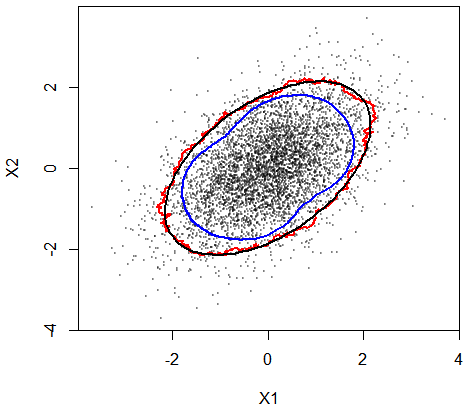
\includegraphics[height=0.15\textheight]{AIStats_fig1a.png} &
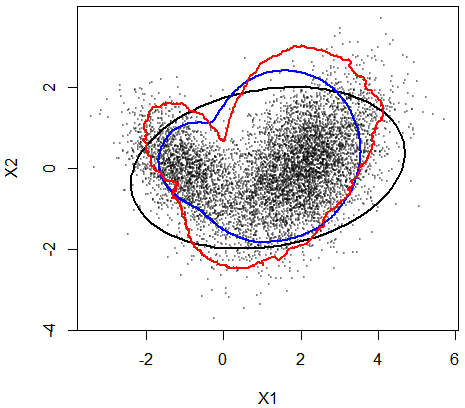
\includegraphics[height=0.15\textheight]{AIStats_fig1b.png} \\
(a) & (b)  \\
%\hline 
\end{tabular}
\caption{Comparison of usual projection quantiles (blue) 
with weighted projection quantiles (red), 
along with a Gaussian confidence ellipsoid (black) for a Gaussian scatter in (a) 
and mixture of Gaussians in (b). 
Areas under the different curves are not expected to 
be equal.}
\label{fig:1}
\end{figure*}
%]

%\begin{figure*}[htb]
%\centering 
%\begin{tabular}{cc}
%%\hline 
%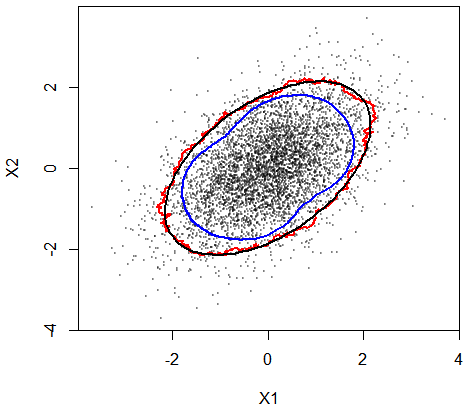
\includegraphics[width=0.45\textwidth,height=0.15\textheight]{AIStats_fig1a.png} &
%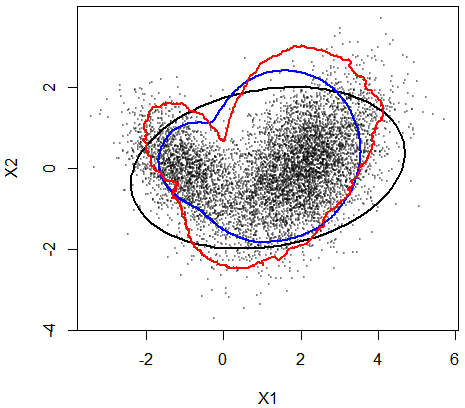
\includegraphics[width=0.45\textwidth,height=0.15\textheight]{AIStats_fig1b.png} \\
%(a) & (b)  \\
%%\hline 
%\end{tabular}
%\caption{Comparison of usual projection quantiles (blue) 
%with weighted projection quantiles (red), 
%along with a Gaussian confidence ellipsoid (black) for a Gaussian scatter in (a) 
%and mixture of Gaussians in (b). 
%Areas under the different curves are not expected to 
%be equal.}
%\label{fig:1}
%\end{figure*}
%%]

We discuss below how the sets of Figure~\ref{fig:1}, 
 and their enclosing boundary curves, may be indexed by vectors of the 
unit sphere in the feature space. 
Curves and enclosed sets as in Figure~\ref{fig:1} are fast and accurate visualization 
tools that are easily available from the proposed procedure. These graphical techniques 
are naturally best suited for two and three dimensional projections of the data, however, 
the construction of such sets in any dimension is simple and quick in our proposed 
methodology. We can take full advantage of distributed and parallel computing tools 
for  this purpose, since the constructions of sets like the ones depicted in 
Figure~\ref{fig:1} is linear in both dimension ($p$) of the feature space, and 
the number of observations ($n$), and parallelizable in both dimensions and sample size. 
Since the DCW is central to the geometric learning procedure, 
we present theoretical properties of it 
in Section~\ref{sec:DCWTheory}.  

We also use the DCW algorithm to compute the {\it data-depth} of any point 
in the feature space, with respect to any probability distribution function, or data 
cloud. A data-depth is a relative measure of how close is the given point in space 
to the center 
of a data cloud or a median of a (multivariate) probability distribution function. 
We discuss technical results of data-depths in the current context in 
Section~\ref{sec:DataDepth} below. The crucial 
component of obtaining the 
depth of a given point with respect to a cloud of observations is to project the 
observations {\it in a single direction}, 
which is extremely fast and easy, apart 
from being an embarrassingly parallel procedure. 



One immediate application of the DCW  and the related data-depth algorithm 
is in supervised learning, presented in Section~\ref{sec:GLA}.
Owing to the 
speed and efficiency of the DCW and data-depth algorithms, such classification of 
observations can be carried out extremely quickly, and the proposed 
{\bf geometric learning} procedure may 
be used for {\it online supervised learning}. Thus, this can be adapted for 
a real-time analytics tool
for classification in big data. Moreover, since we do not make assumptions about 
the geometry of the description of the data cloud $\mathbf{X}_{k}$ for any $k$, 
the proposed procedure is {\it robust} against failures of statistical assumption. 
Note that
most statistical assumptions are essentially unverifiable declarations in 
high-dimensional data, hence such robustness properties are essential. 

Apart from being fast and robust, the geometric learning procedure is surprisingly 
versatile and efficient. In the different datasets we have analysed, some 
of which are presented below, 
it seems that the proposed procedure is competitive, if not better, than standard 
supervised learning methods that are in popular usage. 
Results are presented in Section~\ref{sec:DataAnalysis} for some 
simulated data examples, and in Section~\ref{sec:RealData} for two real data examples, one of which 
is a high-dimensional classification problem. We conclude this 
paper with Section~\ref{sec:Conclusions}, where we present some caveats about using 
geometric learning, and some future research directions.




%
%All statistical supervised learning procedures, 
%either explicitly or implicitly, 
%operate under the assumption that the conditional distribution of the feature 
%$X$ given label $Y = y$ (in notations: $[X | Y = y]$), is 

 
\section{The projection quantile} 
\label{sec:PQ}

We denote the  open unit ball in $p$-dimensional Euclidean plane as 
$\mathcal{B}_{p} = \{ x  \in \mathbb{R}^{p}: || x || < 1 \}$. The notation 
$|| \mathbf{a} ||$ stands for the Euclidean norm of a vector $\mathbf{a}$, while 
$\langle \mathbf{a}, \mathbf{b} \rangle$ 
stands for the Euclidean inner product between two vectors.
For convenience, we reserve the notation 
$\mathbf{0}$ for a vector of zeroes, and $\mathbf{1}$ for a vector of ones, in appropriate 
dimensions that will be specified in the right contexts. 
Also, we reserve the notation $\mathbf{u}$ to 
denote a typical element in this open unit ball. 
We further reserve the notation $\mathbf{e}_{\mathbf u}$ 
for the unit vector in the direction of 
$\mathbf{u} \in \mathcal{B}^p$. Thus,  $\mathbf{e}_{\mathbf u}  = 
\frac{\mathbf{u}}{||\mathbf{u}||}$ when 
$\mathbf{u} \ne \mathbf{0} \in \mathbb{R}^{p}$ and 
$\mathbf{0}$ otherwise.
For any vector ${x} \in \mathbb{R}^{p}$, we define 
${x}_\mathbf{u} = \langle {x}, \mbfeu \rangle$.
The projection of ${x}$ in the direction of $\mathbf{u}$ is,
${x}_\mathbf{u} \mbfeu 
= ||\mathbf{u}||^{-2} \langle \mathbf{x}, \mathbf{u} \rangle \mathbf{u}$. 


Let ${X} \in \mathbb{R}^p$ be a random variable in $p$-dimensional Euclidean 
space. 
For the moment, assume that the center of the distribution of ${X}$ 
is the origin. 
Let, $\mathbf{q}_\mathbf{u}$ be the $ (1 + || \mathbf{u} ||)/2$-th quantile of 
${X}_\mathbf{u}$, that is, 
$\mathbb{P} [ {X}_\mathbf{u} \leq \mathbf{q}_\mathbf{u} ] = 
(1 + || \mathbf{u} || )/2$. The $\mathbf{u}$-th projection quantile (PQ) is defined 
in \cite{MukhopadhyayC11} as
\begin{equation}
Q_{proj} (\mathbf{u}) = \mathbf{q}_\mathbf{u} \frac{\mathbf{u}}{||\mathbf{u}||} 
= \mathbf{q}_\mathbf{u} \mbfeu.
\end{equation}

\begin{figure*}[htb]
\centering 
\begin{tabular}{|c|c|c|}
\hline 
\includegraphics[width=0.3\textwidth,height=0.15\textheight]{../../../../Programs_Umn_Stat/Current/Quantiles/fig5.pdf} &
\includegraphics[width=0.3\textwidth,height=0.15\textheight]{../../../../Programs_Umn_Stat/Current/Quantiles/fig7.pdf} &
\includegraphics[width=0.3\textwidth,height=0.15\textheight]{../../../../Programs_Umn_Stat/Current/Quantiles/fig10.pdf} \\
(a) & (b) & (c) \\
\hline 
\end{tabular}
\caption{A graphical depiction of the quantile function in one and two dimensions}
\label{fig:2}
\end{figure*}

The {\it sample} version of a projection 
quantile, when data $\{ X_{1}, \ldots, X_{n} \}$ are available, is defined 
exactly as above, in terms of the empirical distribution function 
$\mathbb{F}_{n} (\cdot) = n^{-1} \sum_{i=1}^{n} I_{\{ X_{i} \leq \cdot \}}$, where 
$I_{A}$ for any measurable set $A$ is the indicator variable denoting whether $A$ holds
or not. 
Note that the data cloud ${X}_{1}, \ldots, {X}_{n}$ needs to be centered 
to apply the above technique. 
 The co-ordinatewise median (the 0.5 quantile) of the data cloud acts as a good choice of the center. 
 
The projection quantile has several interesting properties, which makes it 
attractive from both theoretical and algorithmic points of view. 
It is  linearly 
dependent on the number of dimensions $p$  in 
calculation of ${X}_\mathbf{u}$. The sample PQ computation is linear in $n$ also. 
Additionally, it can be easily seen that the computation of projection quantiles 
in different directions are unrelated to each other, and can be trivially distributed
over a network of computing cores. 

We present a brief motivation of the above PQ here, by using the illustrative example of 
univariate and bivariate Gaussian random variables. Note that for a real random 
variable $X$, 
the quantile function is defined on the interval $[0, 1]$ of probabilities and has as 
its range as the support of the random variable, and is traditionally defined as 
$Q (a) = \inf \{ q: \mathbb{P} [ X \leq q ] \geq a \}$ for any $a \in [0,1]$. For the 
standard Gaussian distribution, this is illustrated in the left panel of 
Figure~\ref{fig:2}. Note, however, the following is also true 
\cite{Ferguson67, Chaudhuri96}:

\begin{Theorem} 
The $a^{th}$ quantile is the smallest minimizer of the function 
$\mathbb{E} \left[ | X - q| + (2 a - 1) (X - q) \right]$. 
\end{Theorem} 

Existence and uniqueness of $Q (a)$ is not an issue, owing to convexity of the 
criterion function, and hereafter we assume adequate conditions to ensure that in
the {\it population}, the above convex criterion function has a unique minimizer. 
Assuming that the random variable $X$ is absolutely continuous is sufficient 
for this purpose, and hereafter we assume all feature vectors are absolutely continuous 
random variables.



In view of the above, we may alternatively define the quantile 
function as being indexed by $u = 2 a - 1 \in [-1, 1]$, and $Q (u)$ as the 
(unique) minimizer of the convex function 
$\mathbb{E} \left[ | X - q| + u (X - q) \right]$, as illustrated by the 
middle panel in Figure~\ref{fig:2}. This definition of a quantile function was extended 
by \cite{Chaudhuri96} for $p$-dimensional random variables as being indexed 
by vectors 
 $\mathbf{u} \in \mathcal{B}_{p} = \{ x  \in \mathbb{R}^{p}: || x || < 1 \}$, and 
 defined as minimizers $Q (\mathbf{u} )$ of 
$\mathbb{E} \left[ || X - q|| + <\mathbf{u},  X - q> \right]$, as illustrated in the 
right panel of Figure~\ref{fig:2}. This is a generalization of one of the 
earliest attempts at defining multivariate median by \cite{Haldane48}.
Note that Chaudhuri's multivariate quantiles cannot be 
computed for $p > n$ using the algorithm given in \cite{Chaudhuri96}, and requires
iterative methods for even $p \leq n$. 
Additionally, it was seem that ($a$) this definition of 
multivariate quantiles does not capture the data geometry adequately, and ($b$) 
$Q (\mathbf{u})$ and $\mathbf{u}$ were nearly parallel in several simulated data examples. 
These observations motivate the projection quantile, where instead of using 
the full Euclidean norm of $X - q$, we only use that part of $X - q$ that is parallel 
to $\mathbf{u}$. Some amount of algebra reduces this procedure to the description 
of PQ provided above, and Figure~\ref{fig:1} shows its efficacy. 


 
 
 \section{The data cloud wrapper}
 \label{sec:DCWTheory}
 
The PQ described above does not fully capture the shape of the data geometry, 
mainly because of two issues. First, the spread of the data in different directions 
$\mbfeu$ from the center is different, and PQ does not accomodate for that. Second, 
all information  related to any feature vector $X_{i}$ in the directions orthogonal 
to $\mbfeu$ is discarded. The {\it data cloud wrapper} (DCW) algorithm attempts 
to correct these two discrepancies in the PQ, by introducing two weight functions. 
First, we adjust the {\it direction specific scaling} using $w_{\mathbf{u}}$ 
defined below. Then, we incorporate the information from the $i^{th}$  observation 
in the directions orthogonal to $\mbfeu$ using another weight factor $w_{2i}$, also 
detailed below.
 
 Recall that in accordance with the notation developed 
 earlier, $X_{\mathbf{u} i} \mbfeu$ is the projection of $X_{i}$ along 
 $\mbfeu$.  After centering (at the coordinatewise median) and scaling (using the 
 median absolute deviation) the data, we first compute 
 $Q_{proj}( \mathbf{u} )$, the projection quantile along $\mathbf{u}$. 
We then compute global weights for the direction vector $\mathbf{u}$ by $k$-mean 
distance. Define $d_i$ is the Euclidean distance of $X_i$ from 
$Q_{proj} (\mathbf{u})$, and $d_{(1)} < \ldots < d_{(n)}$ are the ordered distances. 
We then define the $k$-mean distance as
$\bar{d}_k = \frac{1}{n} \sum_{i = 1}^n d_i \mathbb{I}_{ \{d_i < d_{(k)} \} }$.
Here, $k$ is a tuning parameter that we choose depending on the application. 
We then define $w_{\mathbf{u}} = \exp (- a \bar{d}_k)$ as a scaling  factor to be used 
in the direction $\mbfeu$. 
Our next step is to compute the norms of the vectors 
 $|| X_{\mathbf{u} \perp i} || = || X_i - X_{\mathbf{u} i} \mbfeu ||$, 
 which we use in the weight function
$ w_{2i} = 
\exp \left[ -b \frac{ || X_{\mathbf{u} \perp i}||}{ || X_i ||} \right] 
\mathbb{I}_{ \{ || X_{\mathbf{u} \perp i} || \leq \epsilon \}}$. 
Here, $b$ and $\epsilon$ are tuning parameters.
Suppose $\{ j_{1}, \ldots, j_{n_{u}} \}$ are the indices for which $w_{2 i}$ is non-zero. 
We now define $\tilde X_{\mathbf{u} j_{k}} = 
w_{\mathbf{u}} w_{2 j_{k}} X_{\mathbf{u} j_{k}}$, 
for $k = 1, \ldots, n_{u}$.
The DCW in the direction $\mbfeu$ is obtained by selecting the 
$\alpha = (1 + ||\mathbf{u} ||)/2$-th quantile of 
$\tilde X_{\mathbf{u} j_{1}}, \ldots, \tilde X_{\mathbf{u} j_{n_{u}}}$. 
Let it be $\tilde{q}_\mathbf{u}$. The DCW is the direction $\mbfeu$ is defined as 
$\tilde Q_{proj} (\mathbf{u}) = \tilde{q}_\mathbf{u} \mbfeu$.



In order to state the theoretical properties of the DCW, first
define $\tilde X_{\mathbf{u} i} = 
w_{\mathbf{u}} w_{2 j_{k}} X_{\mathbf{u} i}$, for $i =1, \ldots, n$.  
Also, consider the following two functions
\begin{eqnarray*}
\Psi_{\mathbf{u}} (X, q) &  = & 
\mathbb{I}_{ \{ || X_{\mathbf{u} \perp i} || \leq \epsilon \}} 
\left[ | \tilde X_{\mathbf{u} i}  - q | + ||\mathbf{u}|| (\tilde X_{\mathbf{u} i}  - q ) 
\right], \\
g_{\mathbf{u}} (X, q)  & = &
\mathbb{I}_{ \{ || X_{\mathbf{u} \perp i} || \leq \epsilon \}} 
\left[ \left( 2 \mathbb{I}_{ \{ \tilde{X}_{\mathbf{u} i} \leq q \}} - 1 \right)
- ||\mathbf{u}|| \right].
\end{eqnarray*}
Our results are based on the {\it population level} properties of 
the functions $\Psi_{\mathbf{u}} (X, q) $ and $g_{\mathbf{u}} (X, q)$, that is, 
their behavior when we take an expectation of these functions with respect to 
the measure extended by $X$. Such properties are not assumed for sample level 
functions. 
 An extremely easy 
example where population and sample values differ 
may be seen in the context of a Binomial $(n, \theta)$ random variable $Z$. Note that 
the expectation of $Z/n$ is $\theta$, which is a smooth function on $(0, 1)$. However, 
the sample expectation, ie, the same functional computed under the empirical distribution 
function, is just $Z/n$, which is supported only on discretely many values, and is not 
a smooth function. 



We assume that $\mathbb{E} \Psi_{\mathbf{u}} (X, q) $ is finite for all potential choices 
of $q$, and has a unique minimizer, which we call $q_{\mathbf{u}}^{*}$.
This merely states  that there is a unique population parameter to estimate. 
The sample version does not require uniqueness, but 
that may be enforced, as is traditionally done,  by defining the minimizer to be the infimum over all possible values at which the minimum is reached.
In this framework, we have the following results:

 
\begin{Theorem} \label{thm:Consistency}
The sample DCW is a consistent estimator of the population DCW, that is 
 $q_{\mathbf{u}} \rightarrow q_{\mathbf{u}}^{*}$ almost surely as 
sample size $n \rightarrow \infty$.
\end{Theorem}

\begin{Theorem} \label{thm:AsyNorm}
Under the additional {\bf population level} conditions that  
$\mathbb{E} g_{\mathbf{u}}^{2} (X, q_{\mathbf{u}}^{*}) < \infty$,  and that
the function
$\mathbb{E} \Psi_{\mathbf{u}} (X, q) $ is twice continuously differentiable 
at $q_{\mathbf{u}}^{*}$ with the second
derivative $H$ being positive definite, then as $n \rightarrow \infty$
\begin{eqnarray*}
n^{1/2} ( q_{\mathbf{u}} - q_{\mathbf{u}}^{*}) 
= - n^{-1/2} H^{-1} S_{n} + o_{P} (1),
\end{eqnarray*}
where $S_{n} = \sum_{i=1}^{n} g_{\mathbf{u}} (X_{i}, q_{\mathbf{u}}^{*})$.  
This implies, in particular, that
$n^{1/2} ( q_{\mathbf{u}}^{*} - q_{\mathbf{u}}^{*})$ is asymptotically Normal, with asymptotic variance
$H^{-1} V H^{-1}$ where $V = {\mathrm Var }\  g_{\mathbf{u}} (X, q_{\mathbf{u}}^{*})$.
\end{Theorem}

The proofs of these results, and other theorems that follow, require considerable 
mathematical details. We present a very brief sketch of the main line of argument 
in the supplementary material, and the details can be made available as needed.
 
 
 \section{Data depth using the DCW}
\label{sec:DataDepth}

We consider the support of the feature vector, ${\cal{X}}$ to be a convex set in $\mathbb{R}^{p}$. 
For any given point $\mathbf{p} \in {\cal{X}} \setminus \{ \mathbf{0} \}$ 
the support of a feature of an absolutely continuous
random vector $X$ with cumulative distribution function $F$, 
we define  the {\it data-depth} as $D (\mathbf{p}, F) = \exp ( - \alpha_{\mathbf{p}})$, 
where $\mathbf{u} = \alpha_{\mathbf{p}} \mathbf{p} / || \mathbf{p} ||$, and 
 $\tilde Q_{proj} (\mathbf{u}) = \mathbf{p}$. We extend this to the point 
 $\mathbf{p} = \mathbf{0}$ by defining $D (\mathbf{0}, F)  = 1$. 
  This essentially means that 
 $\alpha_{\mathbf{p}} \in (0, 1]$ is the norm of $\mathbf{u}$, which has the same direction as $\mathbf{p}$, such that $\mathbf{u}^{th}$ DCW is exactly $\mathbf{p}$. 
 
 
The following properties are available for the data depth function $D (\mathbf{p}, F)$:
\begin{Theorem} 
\begin{enumerate}
\item $D (\mathbf{p}, F)  = 1$ if and only if $\mathbf{p} = \mathbf{0}$. 
\item $D ( t \mathbf{p}, F) \leq D (\mathbf{p}, F)$ for all $\mathbf{p} \in {\cal{X}}$, 
and all $t \in [0,1]$. 
\item The directional derivative of $D (\mathbf{p}, F)$ with respect to 
$\mathbf{p}$ exists. 
\item The depth function $D (\mathbf{p}, F)$ is smooth in te second argument, in the sense 
that the Gateux derivative exists.
\item $D (\mathbf{p}, F) \rightarrow 0$ as $|| \mathbf{p} || \rightarrow \infty$. 
\end{enumerate}
\end{Theorem}
Note that the first two properties are the essential properties of a data-depth, while 
the rest of the results are technical properties that help understand the depth function 
better. 
 
 
 

 
 \section{Geometric classification technique}
\label{sec:GLA}

One immediate application of the DCW  and the related data-depth algorithm 
is in supervised learning. 
Consider a feature vector $X \in {\cal{X}} \subseteq \mathbb{R}^{p}$ for some 
(potentially high) dimension $p$, associated with a label 
$Y \in {\cal{Y}} = \{ 0, 1, \ldots, K-1 \}$. Assumed that the observed data is a 
random sample 
$\{ (X_{i}, Y_{i}) \in {\cal{X}} \times {\cal{Y}} 
 \subseteq \mathbb{R}^{p} \times \{ 0, 1, \ldots, 
K - 1 \} \}$ of such $(X, Y)$ pairs. Here $K$, the total number of labels, is 
assumed known. Without loss of generality, we assume that
observations indexed by $S_{k} = \{ i_{k 1}, \ldots, i_{k {n_{k}}} \}$ share the common
label $Y_{i_{k j}} = k$, for any $k \in {\cal{Y}} = \{ 0, \ldots, K-1 \}$. We assume
that $\cup_{k = 0}^{ K - 1} S_{k} = \{ 1, \ldots, n \}$, and 
$S_{k} \cap S_{\tilde{k}} = \varnothing$ whenever $k \ne \tilde{k}$. We denote the 
$n_{k}$ feature observations corresponding to $S_{k}$ by  
$\mathbf{X}_{k} = (X_{i_{k 1}}, \ldots, X_{i_{k n_{k}}})$.

 We elicit the label of any new or unlabeled feature vector 
$x \in {\cal{X}}$ by computing its depths with respect to the $K$ different 
data clouds of observations $\mathbf{X}_{k} = (X_{i_{k 1}}, \ldots, X_{i_{k n_{k}}})$.
We may then choose the label that corresponds to the highest depth value, or construct
labels using more complex usage of the $K$ depth values obtained for $x$. 
For example, one alternative to simply choosing the highest-depth label would 
be to not classify an unlabeled observation if the maximum depth is below a threshold, 
thus paving the way for potentially extending this algorithm to unsupervised 
and semi-supervised classification problems, which we do not pursue here.

Notice that the geometric learning-based separating boundary between two 
labeled classes in the feature space is essentially the locus of the points where 
the data-depths are equal from both the classes. Thus, the separating curves between 
labeled classes are essentially {\it isodepth curves}. This notion can be extended 
to multiple labeled classes easily, and is of independent interest. 

Nevertheless, note that in order to classify a new or unlabeled observation, it is not 
necessary to obtain the entire isodepth curves. The only computation that needs to 
be performed is to obtain the data-depth {\it in the direction of the unlabeled 
observation} relative to each labeled class, which is  trivially a parallelizable 
procedure requiring at most $n$ one-dimensional projections and few other simple 
computations. This leads to the geometric learning algorithm being very much amenable 
to active learning as well as online learning of class labels. 



It may be noted that existing techniques for supervised learning either impose shape 
restrictions explicitly or tacitly, or suffer from  curse of dimensionality, or are 
slow, sequential procedures requiring multiple passes through the data. 
Many methods of supervised learning suffer from multiple of these issues. 
For example, methods like logistic regression for two or more class labels, as well as 
linear or quadratic 
discriminant analysis explicitly make parametric statistical assumptions, which imply 
strong restrictions on the shape of the allowed data layout. The classical version of 
these algorithms are inapplicable for data in high dimensions, and require additional 
assumptions, typically of sparsity of some functional of the feature vector 
distributions, for usability in big data. Some of these additional assumptions are 
unverifiable in data. Nearest neighbor rules 
implicitly make similar assumptions with a choice of metric and tuning parameters, while 
support vector machines make an implicit choice of allowable geometry using the kernel 
function. Methods like (multivariate) density estimation and subsequent learning 
procedures suffer from the curse of dimensionality. Decision trees and ensemble-based 
methods like classification and regression trees, bagging, random decision forests, 
boosting require iterative and often sequential computation, and may impose shape 
restrictions on the data and may suffer from curse of dimensionality depending on the 
algorithmic details. 

 
 \section{Geometric learning example: simulated data}
 \label{sec:DataAnalysis}
 
In this section we use two simulated datasets to demonstrate the key 
characteristics of the proposed geometry learning algorithm, and compare 
its performance with state-of-the-art alternatives.  



%
%\begin{figure}[h]
%\includegraphics[width = 0.45 \textwidth]{QuantClassifier1.png}
%\includegraphics[width = 0.45 \textwidth]{WPQSimul2Pic2.png}
%
%%\begin{figure}[H]
%%\includegraphics[width=0.99\textwidth]{WPQSimul1Pic3.png}
%%\caption{Scatterplot of Simulated Dataset 1 with Class Separator by the Proposed Geometric Classification Method and Other Standard Methods}
%%\label{fig:SimulatedExample3}
%%\end{figure}
%%
%%
%%
%%%\begin{figure}[H]
%%%\includegraphics[width=0.99\textwidth]{WPQSimul2Pic1.png}
%%%\caption{Scatterplot of Simulated Dataset 2 with Class Separator by the Proposed Geometric Classification Method}
%%%\label{fig:SimulatedExample4}
%%%\end{figure}
%%
%%\begin{figure}[H]
%%\includegraphics[width=0.99\textwidth]{WPQSimul2Pic2.png}
%%\caption{Scatterplot of Simulated Dataset 2 with Class Separator by the Proposed Geometric Classification Method and the Iso-depth Contours}
%%\label{fig:SimulatedExample5}
%%\end{figure}
%%
%%\begin{figure}[H]
%%\includegraphics[width=0.99\textwidth]{WPQSimul2Pic3.png}
%%\caption{Scatterplot of Simulated Dataset 2 with Class Separator by the Proposed Geometric Classification Method and Other Standard Methods}
%%\label{fig:SimulatedExample6}
%%\end{figure}
%
%\caption{Quantile Datadepth Based Iso-depth Seperation Curves for a Binary Classification Problem}
%\label{fig:SimulatedExample}
%\end{figure}

%The data in the example is generated from a mixture of bivariate normal data. 


\begin{figure*}[htb]
\vspace{0.05cm}
\centering 
\begin{tabular}{| c | c |}
\hline 
\includegraphics[width = 0.45 \textwidth,height=0.18\textheight]{QuantClassifier1.png}
&
\includegraphics[width = 0.45 \textwidth,height=0.18\textheight]{WPQSimul2Pic2.png}\\
(a) & (b)  \\
\hline 
\end{tabular}
\caption{Isodepth separation curves for a binary classification problem 
in two datasets}
\label{fig:SimulatedExample}
\end{figure*}

The simulated data contains two classes, and is depicted in 
Figure ~\ref{fig:SimulatedExample} with black and red points.  
We present the two simulated datasets in this figure, in the two panels.
In both panels, the black points are clustered in the apple shaped figure, while 
 the red points are in the top leaf cluster. The dotted lines in green and black 
 are the DCW curves corresponding to the black and red observations respectively, 
 corresponding to $|| \mathbf{u} || = 0.9$. The solid blue curve indicates the 
 iso-depth curve for this dataset, which acts as the curve of separation for the 
 two groups of data. In order to evaluate the classification accuracy 
 and speed of our algorithm, we 
 randomly selected $80 \%$ of the observations from each group for training, 
 and evaluated the 
 geometric learning algorithm on the rest $20 \%$ test data from each group. 
 For comparison purposes, 
 we also used several standard classification algorithms on identical training 
 and testing datasets. 
  This process was repeated 1000 times to ensure sufficient randomization. 
The running time are based on running each of the methods on a 1 GHz, quadruple core computer in R 3.1.1 platform. We present the classification accuracy results in 
 Table~\ref{table:ComparisonTable}. 
 
  
 As can be seen from  Table~\ref{table:ComparisonTable}, the geometric learning algorithm 
is comparable or better in terms of classification accuracy and speed compared to the 
state-of-the-art methods. 
In fact, it is considerably fast in comparison to the other algorithms 
which achieve similar levels of accuracy in different datasets, of which we have 
chosen two illustrative examples. In particular, the geometric learning technique is 
considerably faster than random forest and support vector machines (SVM), and 
slightly faster than the $k$-nearest neighbor (KNN) algorithm. 
In general, parametric methods like linear or quadratic discriminant analysis (LDA, QDA), 
and logistic regression, or procedures like  neural networks do not achieve 
a good class separator, especially in dataset (b) where the classes are 
not as distinct as in case of dataset (a). 

We used the standard packages and routines in the open source software {\tt R}, namely 
{\tt glm, lda (MASS), qda (MASS), randomForest, svm (e1071), nnet, knn (class)}
for the existing supervised learning methods reported here. 
In the random forest procedure, the number of trees for each run was kept at 500, 
sampling was done with replacement, and the rest of the parameters 
were run with default setting. Radial basis kernel 
($ = \exp ( - \gamma | u - v |^2 ) $) was used for the SVM fit of type \textit{C-Classification} using a scaling of $1$ and a class weight 
equal to the proportion of observation in each class in the train set. 
For neural nets, the size of the hidden layer was set at 2, case-wise sample 
weights were set at 1, and entropy fit was used. 
More details on the classification techniques 
used for our analysis, and detailed graphical results from this simulation study may 
found in the supplementary material. Algorithmic and statistical details of 
these learning techniques can be found in \cite{HTF09}.

 


\section{Performance of the Algorithm on Standard Datasets}
\label{sec:RealData}


We show the performance of the dataset on two multiclass multivariate datasets, namely 
the celebrated
Fisher's iris dataset,  and the colon dataset from the {\tt R} package {\tt cepp}. 


\subsection{Fisher's Iris Dataset}

This is perhaps the best known dataset to be found in the 
pattern recognition, learning and statistical classification literature. 
Performance on this dataset is a litmus test for any new proposed 
machine learning method. The data contains three classes of Iris plants
 of 50 instances each. The three classes are {\it Iris setosa}, 
 {\it Iris versicolor} 
 and {\it Iris virginica}. There are four features related to the Iris plant  and flower 
 in this dataset: sepal length, sepal width, petal length and petal width, all 
 in centimeters. We use the same methods and techniques as in the simulated 
 data analysis discussed above. 
 
 
 

In Table~\ref{table:IrisTable} we present the average classification accuracy 
in the test data sets from the Iris data.  The running time of all the algorithms 
are very similar since the dataset is small with 150 observations and 4 predictors.
In terms of performance, while all methods perform well, the proposed Geometric Learning
algorithm is the second best, beaten only marginally by the $k$-nearest neighbor method. 


\subsection{Classifying big data: the colon cancer dataset}

The colon dataset is a publicly available dataset for $n = 62$ individuals related to 
colon cancer. This dataset was generated using Affymetrix oligonucleotide arrays, and  
contains expressions levels for 40 tumor and 22 normal colon tissues. Out of the 
originally measured 6500 human genes, $ p = 2000$ with the highest minimal intensity 
across the tissues are selected for classification purposes. Each score represents a gene 
intensity derived in a process described in \cite{Alonetal99}. Note that in this case 
dimension $p$ is considerably higher than sample size $n$, and thus represents a big 
data  supervised learning problem.

%%%% Dropping this for now since we need to read and understand what they are doing
%
% Furey et. al (2000) analyzed the same data and achieved a minimum misclassification of 6 
%observations in a similar process of leave one out classification. We present the output 
%for our analysis of the same data in Table \ref{table:ColonTable}.


It can be seen that the Geometric Learning Algorithm is the most successful among the 
supervised learning methodologies that were usable for this dataset, both in terms 
of prediction accuracy, as well as n terms of speed. Methods not reported 
here were not applicable without additional unverifiable technical 
assumptions. Support vector machines perform marginally better in terms of accuracy, 
but requires an 80-fold increase in computing time. The $k$-nearest neighbor method 
has comparable accuracy to Geometric Learning, but requires nearly $7$-fold more run 
time for each single choice of $k$, and the performance is dependent on the choice of $k$.
For example, we ran the $k$-nearest neighbor algorithm for  $k = \{ 1, \ldots, 15 \}$, 
to obtain the best performance of this method, consequently the actual 
process time should be multiplied by 15, and is thus about a $100$-fold more than 
Geometric Learning. 
Figure \ref{fig:KnnAccuracy} shows the dependence of KNN on different values of $k$. 



%%%%%%%%%%%%%%
%%%%%%%%%%%%%% I have dropped the Foley et all reference for the
%%%%%%%%%%%%%% colon data, since I'm not sure if they are reporting test data only.
%%%%%%%%%%%%%%
%%%%%%%%%%%%%%



\section{Conclusions and future directions}
\label{sec:Conclusions}

The geometric learning algorithm can be seen to be very versatile, and applicable in 
complicated supervised learning problems, as well as in high dimensions. 
One future research to pursue is on theoretical quantification of its classification 
error bound. Another important consideration in this line of research is to evaluate its 
performance in unsupervised learning problems. 

Some of the limitations of the geometric learning method arise from the topological 
restrictions it imposes on the data corresponding to any labeled class. While such 
restrictions are minimal, it is nevertheless unlikely to succeed in classification 
problems where the data cloud for any class consists of more than one connected 
component, or have genus greater than zero. We can envisage how to extend the geometric
learning algorithm to address these kind of data features, but nevertheless additional 
research needs to be carried out. 







%\onecolumn
%\newpage

%\begin{figure}[htb]
%\centering 
%\begin{tabular}{cc}
%%\hline 
%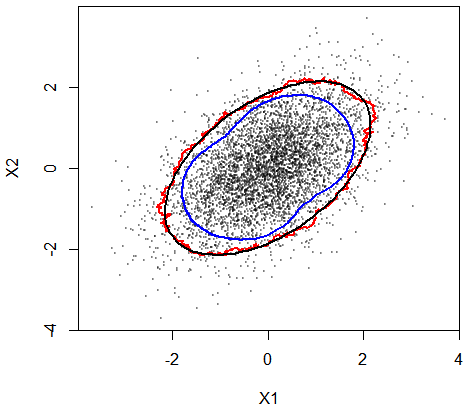
\includegraphics[width=0.45\columnwidth,height=0.15\textheight]{AIStats_fig1a.png} &
%%\includegraphics[width=0.3\columnwidth,height=0.3\textheight]{../../../../Programs_Umn_Stat/Current/Quantiles/fig7.pdf} &
%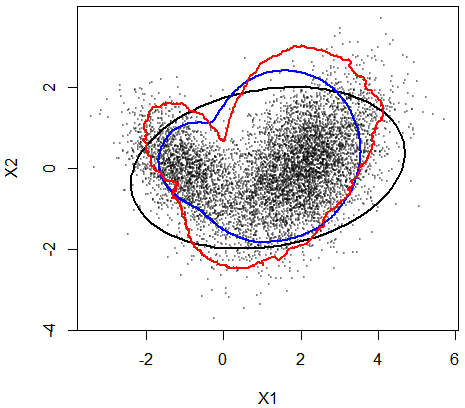
\includegraphics[width=0.45\columnwidth,height=0.15\textheight]{AIStats_fig1b.png} \\
%(a) & (b)  \\
%%\hline 
%\end{tabular}
%\caption{Comparison of usual projection quantiles (blue) 
%with weighted projection quantiles (red), 
%along with a Gaussian confidence ellipsoid (black) for a Gaussian scatter in (a) 
%and mixture of Gaussians in (b). 
%Areas under the different curves are not expected to 
%be equal.}
%\label{fig:1}
%\end{figure}
%
%
%\vspace{0.15cm}
%
%\begin{figure}[h]
%\centering 
%\begin{tabular}{|c|c|c|}
%\hline 
%\includegraphics[width=0.3\columnwidth,height=0.15\textheight]{../../../../Programs_Umn_Stat/Current/Quantiles/fig5.pdf} &
%\includegraphics[width=0.3\columnwidth,height=0.15\textheight]{../../../../Programs_Umn_Stat/Current/Quantiles/fig7.pdf} &
%\includegraphics[width=0.3\columnwidth,height=0.15\textheight]{../../../../Programs_Umn_Stat/Current/Quantiles/fig10.pdf} \\
%(a) & (b) & (c) \\
%\hline 
%\end{tabular}
%\caption{A graphical depiction of the quantile function in one and two dimensions}
%\label{fig:2}
%\end{figure}
%
%\vspace{0.05cm}

\newpage


\begin{figure*}[t]
\includegraphics[width=0.99\textwidth,height=0.25\textheight]{knncolon.png}
\caption{Correct classification (out of 62 cases) for KNN as a function of the 
choice of $k$ in colon cancer data}
\label{fig:KnnAccuracy}
\end{figure*}



\begin{table*}[h]
\begin{center}
\begin{tabular}{| c| c c || c c |} \hline
\multicolumn{1}{| c }{}
 & \multicolumn{2}{| c |}{ Data (a) }  & \multicolumn{2}{| c |}{ Data (b) } \\ \hline  
Method & Accuracy & Run time  & Accuracy & Run time 
\\ \hline
Geometric learning & 0.996 & 1.46  & 0.976 & 1.48 \\
Logistic regression & 0.981 & 0.28 & 0.901 & 0.31 \\
LDA & 0.969 & 0.22 & 0.881 & 0.20 \\
QDA & 0.992 & 0.27 & 0.974 & 0.21 \\
Random forest (500 trees) & 0.998 & 23.61 & 0.976 & 31.77 \\
Neural network & 0.967 & 4.76 & 0.962 & 3.56 \\
SVM & 0.984 & 6.45 & 0.974 & 8.54 \\ 
KNN & 0.997 & 1.53 & 0.989 & 1.62 \\ \hline
\end{tabular}
\end{center}
\caption{Comparison of several supervised learning algorithms on the simulated example, in randomly selected test sets. The classification accuracy is the 
average proportion of test sets observations correctly classified. 
%The run time is in ????}
}\label{table:ComparisonTable}
\end{table*}

\begin{table*}[h]
\begin{center}
\begin{tabular}{| c | c |} \hline
 Method & Accuracy \\ \hline
Geometric learning & 0.9733\\
LDA & 0.9600\\
 QDA & 0.9667\\
Random forest (500 trees) & 0.9667\\
Neural network & 0.9267\\
SVM & 0.9533\\
KNN & 0.9741\\ \hline
\end{tabular}
\end{center}
\caption{{Performance of different classification algorithms  on 
the Fisher iris dataset }}
\label{table:IrisTable}
\end{table*}

\begin{table*}[b]
\begin{center}
\begin{tabular} {| c | c  c  c|} \hline
Method & \# Mis-classified & Accuracy & Run time \\ \hline
Geometric Learning & 9 & 0.854 & 0.21 \\
%2&Logistic Regression&NA&NA&NA\\
Random forest (500 trees) & 10 & 0.839 & 226.92\\
LDA & 15 & 0.758 & 45.12\\
%5&QDA&NA&NA&NA\\
%6&NNET&NA&NA&NA\\
SVM & 8 & 0.871 & 17.36\\ 
%8&SVM(Furey et. al, 2000)&6&0.903&NA\\
KNN(K=3) & 9 & 0.854 & 1.41\\ \hline
\end{tabular}
\end{center}
\caption{Classification results in the colon cancer data}
\label{table:ColonTable}
\end{table*}

\newpage



\bibliography{AIBIB}
\end{document}
